%% LyX 2.0.6 created this file.  For more info, see http://www.lyx.org/.
%% Do not edit unless you really know what you are doing.
\documentclass[11pt]{article}
\usepackage[latin9]{inputenc}
\usepackage{listings}
\setlength{\parindent}{0cm}
\usepackage{float}
\usepackage{url}
\usepackage{amsmath}
\usepackage{amssymb}
\usepackage{graphicx}
\usepackage{url}

\makeatletter

%%%%%%%%%%%%%%%%%%%%%%%%%%%%%% LyX specific LaTeX commands.
%% Because html converters don't know tabularnewline
\providecommand{\tabularnewline}{\\}

\@ifundefined{date}{}{\date{}}
%%%%%%%%%%%%%%%%%%%%%%%%%%%%%% User specified LaTeX commands.
%
% File acl2013.tex
%
% Contact  navigli@di.uniroma1.it
%%
%% Based on the style files for ACL-2012, which were, in turn,
%% based on the style files for ACL-2011, which were, in turn, 
%% based on the style files for ACL-2010, which were, in turn, 
%% based on the style files for ACL-IJCNLP-2009, which were, in turn,
%% based on the style files for EACL-2009 and IJCNLP-2008...

%% Based on the style files for EACL 2006 by 
%%e.agirre@ehu.es or Sergi.Balari@uab.es
%% and that of ACL 08 by Joakim Nivre and Noah Smith


\usepackage{acl2013}\usepackage{times}\usepackage{url}\usepackage{latexsym}%\setlength\titlebox{6.5cm}    % You can expand the title box if you
% really have to

\title{The Palmisano system: measuring similarity between questions with a Takelab implementation}

\author{Lisa Vitolo \\
  University La Sapienza of Rome \\
  {\tt lisavitolo90@gmail.com} \\
}


\makeatother

\begin{document}
\maketitle 
\begin{abstract}
The Palmisano system is going to be a live Question Answering system operating on Twitter.
Starting from the original question posed by the user, Palmisano searches similar questions,
complete with their answers, from QA databases. Extracted questions need to be evaluated so
that the most similar to the original one is used to generate the final answer. This project
developed a semantic similarity system based on the TakeLab \textit{simple} system, which shall
be used to assign a score to extracted questions, measuring their semantic similarity to the original one.
TakeLab, however, was not designed for tweets, and so I will present a discussion on the possible
issues and improvements for making this an efficient similarity system targeted to Twitter usage.
\end{abstract}

\section{Introduction}

A Semantic Textual Similarity system aims at assigning a degree of semantic similarity to two sentences.
This is a problem that has many applications in the Natural Language Processing field.
It has been presented for the first time as a pilot task in the Semeval 2012 (Task 6), and proposed again in the Semeval 2013.
You can find a list of submitted systems, data and proceedings, in their official page: \url{http://www.cs.york.ac.uk/semeval-2012/task6/}.

\medskip{}

Semantic similarity can be easily seen as a regression problem.
With regression we try to learn a function $f\,:\, X\rightarrow\mathbb{R}$
where X is the sample space, in our case the infinite space of all the possible sentence pairs written in English.
The values of this function are in the real domain. In this problem we actually talk about a restricted domain,
lying in the range [0, 5]. This, however, doesn't affect its nature and possible solutions.

\medskip{}

The remainder of this paper is structured in this way: section number 2 presents the TakeLab simple system,
outlining all of its steps with references to recent works and studies in the field.
The Related work section expands those references in order to give a summary of the state of the art
for semantic similarity. Next, some practical details and issues regarding this project implementation
are presented. Section 5 is concerned entirely with results and comparisons. Finally, section 6 delves
into the task of applying this or similar systems to question answering in Twitter.

\section{TakeLab}
TakeLab \cite{Saric:12} is one of the STS systems presented for solving
the Semeval 2012 task. Using the evaluation measures proposed in the
presentation paper \cite{Agirre:12}, and discussed in the Results, it ranked
among the top fifth.

\medskip{}

As mentioned above, solving the STS problem can be seen as solving
a regression task. TakeLab, like most systems presented for the contest,
embraced the machine learning approach, and Figure 1 shows a quick
scheme of its organization.

\begin{figure}
\begin{centering}
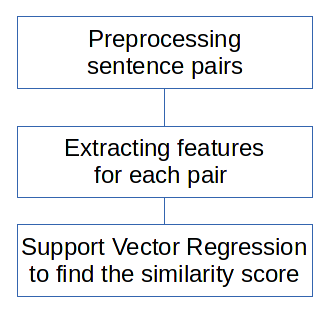
\includegraphics[scale=0.7]{/home/shainer/source/semnlp/src/papers/takelab2.png}
\end{centering}

\caption{Organization of TakeLab\label{fig:Organization-of-TakeLab}}
\end{figure}

TakeLab actually presented two systems, called \textit{simple} and
\textit{syntax}. Their difference lies in the set of features they
use, although some basic features are shared. The \textit{syntax}
system tries to exploit more syntactic dependencies and similarities
(for instance looking at the dependency parse trees). The \textit{simple}
system is more focused on numerical values coming directly from ``bag
of words'' features, or from semantic-related tools such as WordNet.

On average the \textit{simple} system slightly outperformed \textit{syntax},
so I decided to implement this one for the project.

\subsection{Similarity Scores}

Similarity scores range from 0 (totally different sentences) to 5
(identical sentences). This is maintained in my implementation too.

Both the training and test set are shipped with a Gold Standard score
for each sentence pair. However, semantic similarity is a concept
that remains vague and open to discussions or contradictions. {[}CIT{]}
recaps all the issues encountered while annotating.


\subsection{Preprocessing steps}

Before features are extracted, sentence pairs are preprocessed with
the following rules:
\begin{itemize}
\item tokenization, Part-Of-Speech tagging and lemmatization;
\item hyphens and slashes are removed;
\item angular brackets appearing at the beginning or
at the end of tokens are removed;
\item some verb abbreviations typical of the English language, such as ``n't''
(see ``cant''', ``don't'',...), are expanded to their non-abbreviated
form;
\item if a compound word appears as a single token in one sentence, but
as two consecutive tokens in the other, then it is replaced by one
token in both. This is useful since having tokens in common between
the two sentences has a visible effect on more than one feature.
\item stopwords are removed using a small list. Stopwords are words that
are so common in the language that they bear no additional information
about the semantics, and so can be ignored completely without loss
of generality. Additionally, if two sentences have a lot of stopwords
in common, this doesn't increase much their probability of being similar,
so leaving them in place may actually confuse the system.
\end{itemize}
The first step is carried on in two ways: for the user question, by
relying on the preceding stages of the Palmisano pipeline. For the
questions extracted from the database the Stanford Core NLP pipeline
is invoked.

All the other steps are taken care of internally, without use of external
libraries.


\subsection{Features}

An introductive node: the overlap between two generic sets is a measure
of how much elements they have in common. It ranges from 0 (no common
element) to 1 (identical sets). Formally, for sets $S_{1}$ and $S_{2}$
their overlap is defined as:

\[
o(S_{1},S_{2})=2\left(\frac{|S_{1}|}{|S_{1}\cap S_{2}|}+\frac{|S_{2}|}{|S_{1}\cap S_{2}|}\right)^{-1}
\]


where $|S|$ is the set's cardinality.


\subsubsection*{NGram Overlap}

Here we build two sets, one for each sentence, containing all of its
unigrams. The first feature is the overlap degree between these two
sets. The procedure is repeated for consecutive bigrams and trigrams,
that is sequences of 2 and 3 tokens.

\medskip{}


Three additional features are obtained from the same overlaps, but
instead of using tokens as they are found in the sentences I use their
lemmatization. This is not present in the original Takelab implementation,
but it was added by the authors as a later improvement.

\medskip{}


This overlap, or degree of coverage between the two sentences, deals
with ``raw'' words or lemmas. Now we move to more sophisticated
types of coverages, who try to take into account other semantic properties
of the tokens in order to obtain a more realistic value.


\subsubsection*{WordNet-augmented word overlap}

Here we try to take into account different words that have however
a quite close meaning. Such ``closeness'' is measured from the path
length similarity of WordNet. Let's define the WordNet-augmented coverage:

\[
P_{WN}(S_{1},S_{2})=\frac{1}{|S_{2}|}\sum_{w\in S_{1}}score(w_{1},S_{2})
\]


\[
score(w,S)=\begin{cases}
1 & w\in S\\
\underset{w'\in S}{\max}sim(w,w') & w\notin S
\end{cases}
\]


where sim is the path-length similarity mentioned before. The complete
feature is a harmonic mean between the two correspondent coverages:

\[
wawo=harmonic\left(P_{WN}(S_{1},S_{2}),\, P_{WN}(S_{2},S_{1})\right)
\]



\subsubsection*{Weighted word overlap}

Here we assign more importance to words expressing more content inside
a sentence. We define the information content of a token as:

\[
ic(w)=\ln\frac{\sum_{w'}freq(w')}{freq(w)}
\]


It's a measure of how frequently the token appears, compared with
the total frequency of all the possible tokens. In order to obtain
the frequency counts a corpus is needed. The Google Books NGram Corpus
collects and counts tokens from millions of books written in English
over a span of several decades.

Next we define the weighted word coverage of one sentence with respect
to another:

\[
wwc(S_{1},S_{2})=\frac{\sum_{w\in S_{1}\cap S_{2}}ic(w)}{\sum_{w'\in S_{2}}ic(w')}
\]


The feature added here is again an harmonic mean:

\[
wwo=harmonic(wwc(S_{1},S_{2}),\, wwc(S_{2},S_{1}))
\]



\subsubsection*{Vector space sentence similarity}

In computational linguistics, the distributional hypothesis states
that words that tend to appear in the same contexts are likely to
be similar; this hypothesis is usually confirmed by the trends in
human annotations. In TakeLab, words and the contexts are expressed
with a term-document matrix. Word vectors are then summed together
in order to compose sentence vectors. The first feature is a cosine
similarity between the two sentence vectors. For the second feature,
word vectors are weighted with the information content of the word
before creating the sentence vectors.

Since the information content is considered a reliable measure of
the importance of one word inside the sentence, it is natural to weight
another feature with it.


\subsubsection*{Normalized differences}

Two normalized differences between the sentences are added: sentence
length and aggregate word information content.

\[
slen=\frac{|len(S_{1})-len(S_{2})|}{\max\left(len(S_{1}),\, len(S_{2})\right)+e^{-5}}
\]


and similarly for the sum of all the information contents.


\subsubsection*{Number overlaps}

This describes three features dealing entirely with numeric tokens,
on the basis that the human annotators for the training set often
gave low similarity scores to sentence pairs where the numbers differed
a lot.


\subsubsection*{Named Entity features}

Two types of Named Entity have been considered: words starting with
a capital letter, and stock index symbols. In the first case of course
there is a loss of precision due to the fact that not all words starting
with a capital letter are actually named entities, but perhaps the
authors thought it was a good tradeoff with respect to using an external
recognizer.

\medskip{}


Among the training sets provided for the contest, economics seems
to be a recurring topic, and thus stock index symbols are mentioned
in the sentences. Another overlap feature in the system is dedicated
to them.


\subsection{10-fold cross-validation}

The Support Vector Regressor needs some parameters that control its
internal behaviour; their number and nature depends mainly on which
regression algorithm and kernel function is used. Choosing the wrong
parameters can affect the system performances a lot: we want our system
to be able to generalize well to a test set that may be quite different
from the training set. Indeed, cross-validation has been proved an
efficient method in reducing the common issue of overfitting.

In order to identify the best choice of parameters from a span of
alternatives, both the original TakeLab and my implementation use
10-fold cross-validation. Cross validation was performed on an union
of all the training files.

\medskip{}


A k-fold cross validation starts by randomly partitioning the data
into k subsets. k-1 subsets are used to train a model with the current
combination of parameters, while the remaining one is kept aside for
validating it. The training is repeated so that every subset plays
the role of the validation set once; this way, the cross validation
ensures that the performance doesn't depend too much on the initial
random partition. Furthermore, the cross validation tries to create
subsets composed of samples that vary as much as possible in their
target scores.

The mean of the results obtained on the k validation sets (usually
measured in terms of correlation) is the performance measure for that
particular combination of parameters.

This is repeated for all the possible choices of parameters we consider
as options. The final choice used in the application is

\,
\[
\left(\begin{array}{c}
C\\
p\\
\gamma
\end{array}\right)=\left(\begin{array}{c}
1\\
0.02\\
2
\end{array}\right)
\]



\subsection{Support Vector Regression}

Support Vector Regression is a supervised learning technique which
was developed as an extension of support vector machines for regression
problems. Since it's supervised, we assume a given dataset $D=\left\{ (x_{1},y_{1}),...,(x_{n},y_{n})\right\} $
with n input samples drawn from an input space X, and target values
belonging to the real domain.

\medskip{}


The goal of $\varepsilon$-SV regression (the one used in my system)
is finding a function f(x) that has at most $\varepsilon$ deviation
from the real targets $y_{i}$ for all the training data, while at
the same time being as flat as possible. So $\varepsilon$ is the
maximum error the function is allowed to make while giving answers.

Let's start with a linear function f, described as:

\[
f(x)=w\cdot x+b
\]


with $w\in X$, $b\in\mathbb{R}$. Flatness means that we define the
following minimization problem on w:

\[
\min\frac{1}{2}\Vert w\Vert^{2}
\]


subject to

\[
|y_{i}-w\cdot x_{i}-b|\leq\varepsilon
\]


(the constraint on the maximum permitted error). We are assuming that
a function that solves this problem exists, but this is not always
the case, and we may allow some violations of the error constraint.
Introducing slack variables, the new problem formulation is:

\[
\min\frac{1}{2}\Vert w\Vert^{2}+C\sum_{i=1}^{n}\left(\xi_{i}+\xi_{i}^{*}\right)
\]


where C describes the tradeoff between the flatness of f and how much
we tolerate errors above the threshold $\varepsilon$.

Using Lagrange multipliers it can be proved that:

\[
w=\sum_{i=1}^{n}(\alpha_{i}-\alpha_{i}^{*})x_{i}
\]


\[
f(x)=\sum_{i=1}^{n}(\alpha_{i}-\alpha_{i}^{*})(x_{i}\cdot x)+b
\]


where the $\alpha$ values are positive Lagrange multipliers. Note
how w is now completely described with a linear combination of the
training samples, and it's not needed to compute it explicitly. Moreover,
the complexity of the function is independent of the dimension of
the input space X.

At this point we need to generalize the procedure to nonlinear functions.
This can be achieved by simply preprocessing the training inputs $x_{i}$
with a function $\phi$ that brings them into another feature space
F. Then the standard SV regression algorithm is applied. The SVR equations
are rewritten as:

\[
w=\sum_{i=1}^{n}(\alpha_{i}-\alpha_{i}^{*})\Phi(x_{i})
\]


\[
f(x)=\sum_{i=1}^{n}(\alpha_{i}-\alpha_{i}^{*})k(x_{i},x)+b
\]


where k is the kernel function; admissible kernel functions must correspond
to the dot product in some feature space F. Note that now w must be
computed separately. My system uses the radial basis (RBF) kernel:

\[
K(x_{i},x_{j})=e^{(-\gamma\Vert x_{i}-x_{j}\Vert^{2})},\quad\gamma>0
\]



\subsubsection{SVR parameters}

It is now immediate to explain the meaning of the parameters we considered
during cross-validation:
\begin{itemize}
\item p is the threshold, or maximum allowed deviation, $\varepsilon$;
\item C is the tradeoff factor in the minimization problem;
\item $\gamma$ is a parameter of the RBF kernel;
\end{itemize}

\section{Related work}


\subsection{What is similarity?}

\cite{Dekang:98} tried to give a complete and exhaustive
definition of similarity, regardless of the kind of entities involved.
They claim that most existing definitions are too tied to practical
applications or knowledge bases. A meaningful example is the distance-based
similarity: here, the similarity between two terms is measured looking
at the path that joins them in a graph where an edge exists between
each pair of related terms. This idea is very powerful: it posed the
basis for WordNet and other machine-readable resources, but it is
completely tied to the presence of such a network. Additionally, the
concept of ``related'' terms is not so obvious: WordNet itself takes
into account only a limited number of possible relationships between
the synsets, cutting off a whole family of possible paths.


\subsection{WordNet}

Despite its limitations, distance-based similarity measures computed
from WordNet has always played a primary role in the semantic similarity
field. As you have seen, TakeLab is no exception in this. Most similarity
measures start from the so-called path length similarity: two synsets
are related by the number of steps it takes to get from one to the
other. If no path exists, they are completely unrelated. \cite{Budanitsky:01}
present a evaluation of 5 distances based on WordNet path-length.


\subsection{Latent Semantic Analysis}

The distributional hypothesis of Natural Language is exploited by
many similarity systems. They try to express linguistic entities (words,
sentences or documents) as numerical vectors that should represent
what the entity ``talks about''. Usually these vectors are created
automatically from corpora, and stacked together to form document
matrices. \cite{Turner:10} describes the most common vector space models,
underlining how these models are useful in automatically representing
the semantics of concepts.

Broadly speaking, three kinds of matrices are used as semantic models:
\begin{enumerate}
\item \textbf{term-document}: here rows are terms (usually single tokens,
sometimes with a POS tag attached) and columns are documents, e.g.
Web pages. In its most basic form, each element contains a frequency
count of the term in the document. Documents should vary enough in
order to be representatives of several different contexts; they are
treated as simple bags of words, so no syntactic structure is maintained.
However, it is argued, this has not been proved to be a big limitation
for the model.
\item \textbf{word-context}: quite similar to the one above, except that
contexts have a less restricted representation;
\item \textbf{pair-pattern}: each row is a pair of tokens, while the columns
represent possible relationships between them. Readers familiar with
the Semantic Web may find some similarities with how RDF expresses
knowledge about domains.
\end{enumerate}
Such matrices tend to be huge, but also very sparse, since every document
typically employs a small fraction of the total lexicon. Mathematical
techniques such as Single Value Decomposition are usually applied
in order to reduce the total dimensionality while maintaining the
most relevant relationships.

These matrices give immediate information about words co-occurrences
and semantics: we briefly passed over the issue of combining them
together in order to get the same kind of meaningful information for
a sentence (or for a bigger text). \cite{Mitchell:08} presents different compositions
of word vectors into sentence vectors, proving that averaging and
summing are not good techniques because they don't take into account
the syntactical structures words show inside the sentence, and therefore
they end up assigning the same vector to sentences that happen to
share a vocabulary. They propose compositions based on multiplications.

\medskip{}


Having a strong and reliable representations of semantics is useful
in web-searching and information extraction tasks. \cite{Deerwester:90} starts
with an historical way of indexing Web pages: keywords are assigned
to each document to briefly summarize its content. Evaluating a query
(a term, for simplicity) is simply a matter of matching it with the
keywords and return the document(s) with the highest number of matches.
This approach has evident issues: too much terms are synonims, or
are closely related, to be able to rely only on exact matches. Latent
semantics enters here to give an idea of what terms are also only
``implied'' by a query, rather than stated explicitly. If we are
able to say that the occurrence of some words implies a relation with
another word, this word can be added to the keyword list automatically.

With LSA we try to build a ``semantic space'' where term or documents
are placed close if they are related with each other, regardless of
which words appear in the document.


\subsection{Notes on other systems}

Reviewing semantic similarity systems presented for the same contest the machine learning approach
clearly prevails. Furthermore the features tend to be drawn from the
same ideas and studies, although they often differ in the actual formulae.
Below are some of the most interesting ones found in systems other
than TakeLab simple:


\subsubsection*{Syntax-related features}

The relation between syntax and semantics has been deeply explored.
Many systems try to infer a semantic relation from syntactical dependecies,
often using syntax tree or dependency parse tree as machine-readable
representations of syntax. Both TakeLab syntax and \cite{Marsi:13}
 contain good examples of this approach.
 
Specifically in the subject of assessing the similarity of questions extracted
from large QA databases, \cite{Wang:09} describes new syntax-related features which, alone or
combined with more "semantic" ones, achieve better results than simply relying
on bag-of-words values. This improvement remain even if some noise is introduced
in the questions in the form of grammatical errors, typical of many Internet users.
It is not immediate to compare their results with those of TakeLab, however, due to
the difference in their evaluation measures.

\subsubsection*{Random Indexing}

Random Indexing is an alternative to LSA for distributional semantics
which again tries to exploit the co-occurrences of words in the same
documents, used for example by \cite{Wu:13}.

\medskip{}


Cross validation is often proposed as a valid techniques for understanding
which features have the most relevant impact on the final performances,
or which of them can be safely ignored.


\subsection{Dataset gathering and annotations}

When the pilot task on semantic similarity was first approved, the
organizators found out data for sentence semantic similarity are a
scarce resource. Existing sets were either too small, or focused on
assesting the similarity of larger portions of text. \cite{Agirre:12} discusses
in details how these issues were overcomed by building a new dataset,
and their efforts to control the quality of the annotations.


\subsection{The Question Answering approach}

As Palmisano proposes itself to do, semantic similarity has been often
applied to the field of question answering. Given a sufficiently large
QA database, similar questions are searched and compared with the
original question in order to find good answers. \cite{Jeon:05} however
are not satisfied with approaches based on building feature vectors,
typical of most systems. They find they often overfit on the training
data and are hard to scale. Their mostly
relies on information extraction techniques. In a nutshell, if two
different queries have the same click log and retrieval results, they
are likely to be similar. The database is searched extensively in
order to build a huge collection of similar question pairs.

Once the collection of pairs is ready, it is easily interrogated in
order to answer to new queries. Additionally, a pre-existing translation
model can be applied to pairs in order to a infer a similarity model.
The underlying concept is treating the pairs as if they were in different
languages: if we train a translation model with those pairs as data,
it will automatically become a semantic similarity model.

\section{Implementation}


\subsection{External dependencies}

My TakeLab implementation uses the following external libraries:
\begin{itemize}
\item Stanford Core NLP, for tokenization, Part-of-Speech tagging, and lemmatization;
\item WS4j, a library for computing WordNet 3.0 similarity scores. It was
picked because the JAR files includes an internal copy of the database,
thus avoiding the need for external database files;
\item LibSVM is an implementation of Support Vector Machines and Support
Vector Regression, found at \url{http://www.csie.ntu.edu.tw/~cjlin/libsvm/}
and described in detail in \cite{Chang:11}.
\end{itemize}
the lib/ subdirectory in the project root contains the JAR files for
these libraries. The stanford-corenlp-models.jar file is needed to
load the machine learning models used by the NLP pipeline.

\subsection{Sample files}

Training and test files were provided by the Semeval 2012 Task 6,
so that all systems could be evaluated on the same samples. Each sample
file was actually split in two: one text file for the sentence pairs,
called STS.input.<name>.txt, and another with the annotated similarity
scores, named STS.gs.<name>.txt.

In order to simplify command line arguments and I/O operations, the
\texttt{\small{putOutput.py}} script merged the two of them into one
text file organized this way:

\begin{lstlisting}
<sentence1>TAB<sentence2>TAB<score>
\end{lstlisting}


This is also the only format recognized by my application. All the
sample files you see in the subdirectories are already in this format,
but \texttt{\small{putOutput.py}} is available in the src/scripts/
folder should you need to convert new samples.


\subsection{The Google NGram Corpus}

The Google NGram corpus is a huge resource, collecting frequency counts
for English tokens spanning across several decades. Unfortunately
it is not really optimized for a huge sequences of queries, so I applied
some processing steps in order to reduce its volume to a manageable
size, also in terms of occupied disk space:
\begin{itemize}
\item the frequency counts for punctuaction characters were not downloaded,
since their information content is not really relevant for this semantic
task;
\item all the counts for the same token, but different year, were summed
together.
\item each row contains only the token, its POS tag, and the frequency count;
additional information about where the occurrences were found were
deleted.
\item counts have been ``indexed'' by the first two initials. The googlebooks/
directory contains a subdirectory for each initial letter; these subdirectories
contain in turn a text file for each pair of initial letters. So for
instance the a/ folder contains ``aa'' for all the tokens starting
with ``aa'', ``ab'', and so on. A special file oneLetter groups
together 1-character tokens.
\item All the tokens not appearing in an online English dictionary, stored
in the dictionary/ folder, have been ignored. The comparison was case
insensitive. The dictionary is the Ispell English Word Lists, chosen
because it includes inflected forms of verbs and nouns (e.g. plurals).
It can be downloaded from \url{http://wordlist.sourceforge.net/}.
\end{itemize}
These steps were applied using the \texttt{\small{mergeYears.py}}
and \texttt{\small{divideByInitials.py }}Python scripts.

Thanks to this, plus some internal caching, lookups inside the corpus
don't add much overhead to the execution time.

\subsection{Usage}

Refer to the README in the project root directory for instructions
for compiling and running the program.


\section{Results}

The Pearson correlation is used to measure the accuracy of the semantic
similarity system with respect to the Gold Standard annotations. I
compute the correlation for each test file, plus two of the three
aggregate measures described in \cite{Agirre:12}: the ALL correlation
is simply the correlation of all the test samples concatenated together.
The Mean correlation is an average weighted with the number of samples
in each test file.

\medskip{}


In Table 1, my results are compared with the original Takelab results,
found in their presentation paper, and with the baseline for the Semeval
task. The baseline scores are produced using just one feature, a simple
word overlap.

\medskip{}


\begin{table}[H]
\begin{centering}
\begin{tabular}{|c|c|c|c|}
\hline 
 & Mine & Takelab & Baseline\tabularnewline
\hline 
\hline 
\noalign{\vskip\doublerulesep}
MSRpar.txt & 0.64 & 0.73 & 0.43\tabularnewline[\doublerulesep]
\hline 
MSRvid.txt & 0.77 & 0.88 & 0.30\tabularnewline
\hline 
SMTeuroparl.txt & 0.39 & 0.47 & 0.45\tabularnewline
\hline 
SMTnews.txt & 0.40 & 0.40 & 0.39\tabularnewline
\hline 
OnWN.txt & 0.61 & 0.68 & 0.58\tabularnewline
\hline 
\multicolumn{4}{|c}{}\tabularnewline
\hline 
ALL & 0.71 & 0.81 & 0.31\tabularnewline
\hline 
Mean & 0.60 & 0.67 & 0.43\tabularnewline
\hline 
\end{tabular}
\par\end{centering}

\caption{Default implementation}
\end{table}


\medskip{}


It appears that the low results obtained for the SMTeuroparl set are
somewhat expected keeping in mind that systems for such complex tasks
tend to overfit on the format of the training data. The Takelab authors
state that the SMTeuroparl training set differs a lot from the corresponding
test set: the latter tends towards significantly shortest sentences,
and many short identical sentences are repeated multiple times.

\medskip{}


Next, I performed small changes on the system to understand how this
affected its performances. For simplicity, only the new aggregated
correlations were reported.

\begin{table}[H]
\begin{centering}
\begin{tabular}{|c|c|c|c|c|}
\hline 
 & New & Default & Takelab & Baseline\tabularnewline
\hline 
\hline 
ALL & 0.7 & 0.71 & 0.81 & 0.31\tabularnewline
\hline 
Mean & 0.58 & 0.60 & 0.67 & 0.43\tabularnewline
\hline 
\end{tabular}
\par\end{centering}

\caption{C=1, P=1, G=2}
\end{table}


Table 2 shows that a not-so-big variation of P doesn't have an important
influence on average.

\begin{table}[H]
\begin{centering}
\begin{tabular}{|c|c|c|c|c|}
\hline 
 & New & Default & Takelab & Baseline\tabularnewline
\hline 
\hline 
ALL & 0.6 & 0.71 & 0.81 & 0.31\tabularnewline
\hline 
Mean & 0.57 & 0.60 & 0.67 & 0.43\tabularnewline
\hline 
\end{tabular}
\par\end{centering}

\caption{C=1, P=1, G=0.02}
\end{table}


From Table 3: as expected, if also G is changed, it starts to matter.

\begin{table}[H]
\begin{centering}
\begin{tabular}{|c|c|c|c|c|}
\hline 
 & New & Default & Takelab & Baseline\tabularnewline
\hline 
\hline 
ALL & 0.46 & 0.71 & 0.81 & 0.31\tabularnewline
\hline 
Mean & 0.35 & 0.60 & 0.67 & 0.43\tabularnewline
\hline 
\end{tabular}
\par\end{centering}

\caption{C=1000, P=0.02, G=2}
\end{table}


Table 4 shows the biggest variation: C was set to the maximum value
possible. Together with the terrible performances, it also resulted
in a much slower training process. This is understandable looking
at the value of P: the algorithm has to make an effort in order to
keep the error below a quite restrictive threshold for almost all
the training samples. It is my guess that such a complicated task
is eventually managed by overfitting to the slightest details to the
training set, hence the poor results on the test set.

\begin{table}[H]
\begin{centering}
\begin{tabular}{|c|c|c|c|c|}
\hline 
 & New & Default & Takelab & Baseline\tabularnewline
\hline 
\hline 
ALL & 0.56 & 0.71 & 0.81 & 0.31\tabularnewline
\hline 
Mean & 0.42 & 0.60 & 0.67 & 0.43\tabularnewline
\hline 
\end{tabular}
\par\end{centering}

\caption{C=1000, P=1, G=2}
\end{table}


The idea presented in Table 4 is partially verified by the results
of Table 5. Now P was set to the highest possible value too, allowing
some more freedom in the training process. Indeed the training took
place at the usual speed again, but still there is too much overfitting
for good performances.

\begin{table}[H]
\begin{centering}
\begin{tabular}{|c|c|c|c|c|}
\hline 
 & New & Default & Takelab & Baseline\tabularnewline
\hline 
\hline 
ALL & 0.60 & 0.71 & 0.81 & 0.31\tabularnewline
\hline 
Mean & 0.53 & 0.60 & 0.67 & 0.43\tabularnewline
\hline 
\end{tabular}
\par\end{centering}

\caption{No information content features}
\end{table}


\begin{table}[H]
\begin{centering}
\begin{tabular}{|c|c|c|c|c|}
\hline 
 & New & Default & Takelab & Baseline\tabularnewline
\hline 
\hline 
ALL & 0.47 & 0.71 & 0.81 & 0.31\tabularnewline
\hline 
Mean & 0.37 & 0.60 & 0.67 & 0.43\tabularnewline
\hline 
\end{tabular}
\par\end{centering}

\caption{No preprocessing steps apart from tokenization, POS tagging and lemmatization}
\end{table}


It must be noted that results obtained from removing the preprocessing
steps and the features may not correspond entirely to reality. For
a completely accurate comparison I should have run the cross validation
on the new set of features, and then trained the model with the new
parameters. This was avoided simply because the cross validation step
is too much computationally expensive.


\subsection{Issues}

Although I've checked my code with great details and tried to follow
the paper to the word, the results show that my implementation has
slightly worse performances than the original TakeLab. This may be
done to a variety of reasons:
\begin{itemize}
\item the Python code they present for extracting features slightly differs
from the one described in the paper: namely, some features have different
definitions and the preprocessing steps are not applied for every
feature. However, I cannot be sure these are not changes added after
the paper was written;
\item I used different external data: LSA matrix, WordNet library, and Google
NGram Corpus.
\item personal errors.
\end{itemize}

\section{Applying this system in Palmisano}

From now on, I'm going to refer to the original TakeLab simple system.
It is my personal opinion that it will not be suitable for being applied
to Tweets ``as it is'', and I'm going to explain why.

First, some of the features and preprocessing functions were clearly
designed with the specific training set in mind (e.g. the stock index
overlap). When commenting on their results, the authors justify the
poor performances on the SMTeuroparl or SMTnews test sets by observing
that they differ a lot in structure and average length from the training
data. Indeed those scores are pretty close to the baseline, which
expresses the worst possible results. So my guess is that the system
is not meant to be immediately generalized to such a different task
as analyzing Twitter messages and Web questions.

\medskip{}


Keeping Twitter and the Palmisano organization in mind, these are
other issues that in my opinion will reduce the performances of this
particular module:
\begin{itemize}
\item misspelled words: very typical of Twitter messages, but also of famous
QA websites such as Yahoo Answers. Most features in TakeLab rely on
words being spelled the correct way. Hopefully the negative effects
of this will be partially reduced by the normalization stage;
\item again on the subject of misspelling, I noticed that words starting
with a capital letter tend to be immediately tagged as proper nouns
by both Stanford Core NLP and other Part-of-Speech tagging tools.
However, a lot of tweets I've seen use capital letters unduly, causing
the named entity related features to fail.
\item I used Stanford Core NLP instead of ArkTweetNLP because I needed the
lemmatization step. Stanford NLP uses the Penn treebank tagset which
is different from the one in Palmisano. The needed translation surely
subtracts some relevant information in the questions.
\end{itemize}
On top of all, I believe that the system should be enriched with some
features designed for dealing with questions before being inserted
in the Palmisano pipeline. A possible idea is a feature comparing
the motives behind a question (asking for a factual information vs.
a personal opinion, asking for a reason, and so on). Furthermore,
when more annotated tweets are available, the training and cross validation
should be repeated on those. 


\section{Acknowledgements}

I would like to thank Emanuele Bastianelli, Ph.D student at DIAG,
for his help in providing LSA data and cross-validation suggestions.
I would like also to thank David Jurgens for his support, especially
for dealing with the Google Corpus.

\begin{thebibliography}{protectcitename{{Association for Computing Machinery}}1983}

\bibitem[{Agirre} 2012]{Agirre:12} Eneko Agirre, Daniel Cer, Mona Diab, and Aitor Gonzalez-Agirre.
\newblock 2012 \newblock {\em SemEval-2012 Task 6: A pilot on semantic textual similarity.}
\newblock In Proceedings of the 6th International Workshop on Semantic Evaluation (SemEval 2012), in conjunction with the First
Joint Conference on Lexical and Computational Semantics (*SEM 2012). ACL

\bibitem[{Budanitsky and Hirst} 2001]{Budanitsky:01} Alexander Budanitsky and Graeme Hirst.
\newblock 2001 \newblock {\em Semantic distance in WordNet: An experimental, application-oriented evaluation of five measures.}
\newblock In Proceedings of ACL Workshop on WordNet and Other Lexical Resources, Pittsburgh, PA.

\bibitem[{Chang and Lin} 2011]{Chang:11} Chih-Chung Chang and Chih-Jen Lin.
\newblock 2011 \newblock {\em LIBSVM: A library for support vector machines.}
\newblock ACM Transactions on Intelligent Systems and Technology, 2:27:1-27:27.

\bibitem[{Deerwester} 1990]{Deerwester:90} Scott Deerwester and Susan T. Dumais and George W. Furnas and Thomas K. Landauer and Richard Harshman.
\newblock 1990 \newblock {\em Indexing by latent semantic analysis},
\newblock In Journal of the American Society for Information Science.

\bibitem[{Dekang} 1998]{Dekang:98} Dekang Lin.
\newblock 1998 \newblock {\em An information-theoretic definition of similarity.}
\newblock In Proceedings of the 15th international conference on Machine Learning, volume 1, pages 296-304. San Francisco

\bibitem[{Jeon} 2005]{Jeon:05} Jeon, Jiwoon.
\newblock 2005 \newblock {\em Finding Similar Questions in Large Question and Answer Archives.}
\newblock Computer Science Department Faculty Publication Series. Paper 138.

\bibitem[{Marsi} 2013]{Marsi:13} Marsi, Erwin; Moen, Hans; Bungum, Lars; Sizov, Gleb Valerjevich; Gamback, Bjorn; Lynum, Andre.
\newblock 2013 \newblock {\em NTNU-CORE: Combining strong features for semantic similarity.}
\newblock Second Joint Conference on Lexical and Computational Semantics (*SEM), Volume 1: Proceedings of the Main Conference and the Shared Task: Semantic Textual Similarity.

\bibitem[{Mitchell and Lapata} 2008]{Mitchell:08} Jeff Mitchell and Mirella Lapata.
\newblock 2008 \newblock {\em Vector-based models of semantic composition.}
\newblock Proceedings of ACL08: HLT, pages 236-244.

\bibitem[{Saric} 2012]{Saric:12} Saric, F., Glavas G., Karan M., Snajder J., Dalbelo Basic B.
\newblock 2012 \newblock {\em TakeLab: Systems for Measuring Semantic Text Similarity.}
\newblock In Proceedings of the Sixth International Workshop on Semantic Evaluation (SemEval 2012). pp. 441-448. ACL, Montreal, Canada (7-8 June 2012).

\bibitem[{Toutanova} 2003]{Toutanova:13} Kristina Toutanova, Dan Klein, Christopher Manning, and Yoram Singer.
\newblock 2003 \newblock {\em Feature-Rich Part-of-Speech Tagging with a Cyclic Dependency Network.}
\newblock In Proceedings of HLT-NAACL 2003, pp. 252-259. 

\bibitem[{Turney and Pantel} 2010]{Turner:10} Peter D. Turney and Patrick Pantel.
\newblock 2010 \newblock {\em From frequency to meaning: Vector space models of semantics.}
\newblock Journal of Artificial Intelligence Research, 37(1):141-188.

\bibitem[{Wang} 2009]{Wang:09} Wang, Kai and Ming, Zhaoyan and Chua, Tat-Seng.
\newblock 2009 \newblock {\em A syntactic tree matching approach to finding similar questions in community-based QA services.}
\newblock Proceedings of the 32nd international ACM SIGIR conference on Research and development in information retrieval.

\bibitem[{Wu} 2013]{Wu:13} Stephen Wu, Dongqing Zhu, Ben Carterette, Hongfang Liu.
\newblock 2013 \newblock {\em MayoClinicNLP-CORE: Semantic representation for textual similarity.}

\end{thebibliography}
\end{document}
